\documentclass[a4paper,12pt]{article}
\usepackage{graphicx}
\usepackage{float}
\usepackage[T1]{fontenc}
\usepackage{hyperref}
\usepackage{adjustbox}
\graphicspath{ {./images/} }
\pagenumbering{gobble}
\begin{document}
	
\author{Miłosz Wojciechowski}
\title{Frames extractor manual}
\date{\today\\ v0.1}


\maketitle
\pagebreak
\pagenumbering{arabic}
\renewcommand{\labelenumii}{\arabic{enumi}.\arabic{enumii}}

\begin{enumerate}
	\item To get full functionality of this program and receive map visualization follow instructions from GoPro-Telemetry-Extractor before proceeding further. If telemetry extractor isn't prepared, this program will only extract frames from a provided video.
	\item Install Python (at least version 3.9):
	\begin{itemize}
		\item Download python  from \url{https://www.python.org/downloads/}. 
		\item \begin{minipage}[t]{\linewidth}
			\raggedright
			\adjustbox{valign=t}{%
				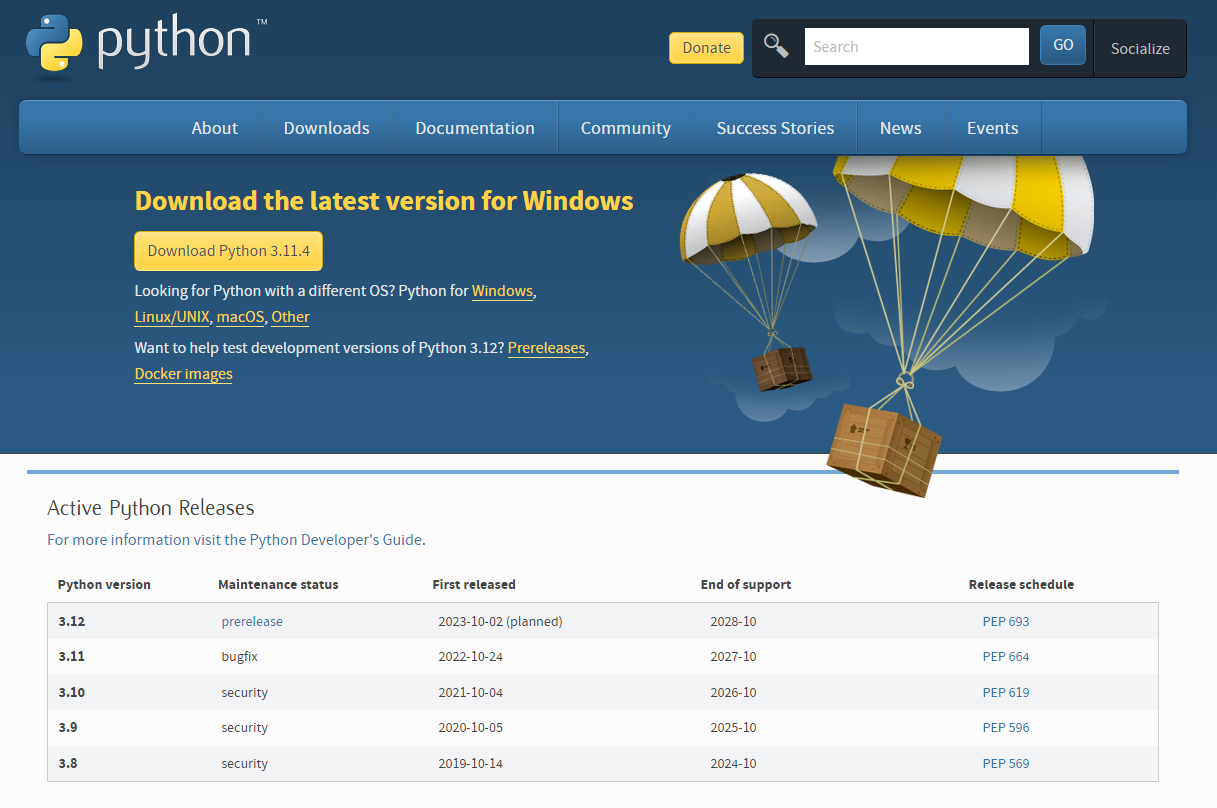
\includegraphics[width=.8\linewidth]{python_install1}%
			}		
			\medskip	
		\end{minipage}
		You can download the latest version by simply pressing the yellow button seen in the picture above. If you want an older version scroll down to the table under "Looking for a specific release?". But not all of them offer installers to download - last python 3.9 release with installer to download is 3.9.13. 
		\item \begin{minipage}[t]{\linewidth}
			\raggedright
			\adjustbox{valign=t}{%
				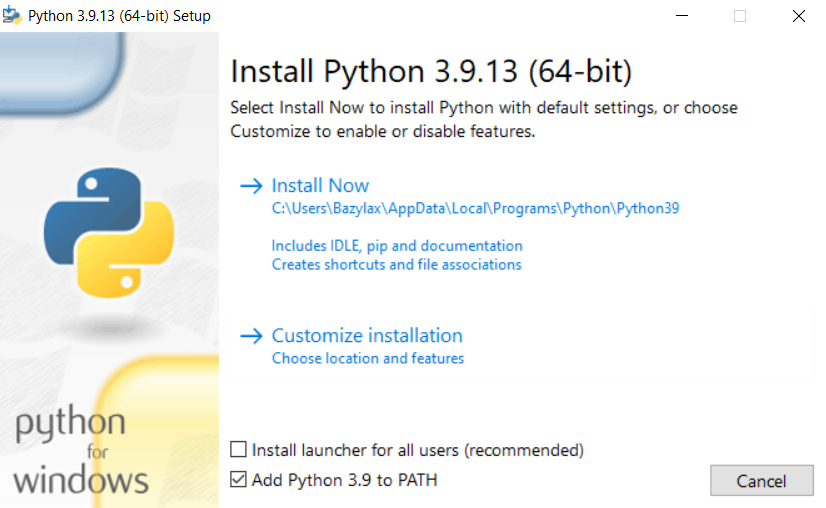
\includegraphics[width=.8\linewidth]{python_install2}%
			}		
			\medskip	
		\end{minipage}
		Choose your installer, either 32-bit or 64-bit depending on your system architecture.
		\item After downloading run the installer
		\item \begin{minipage}[t]{\linewidth}
			\raggedright
			\adjustbox{valign=t}{%
				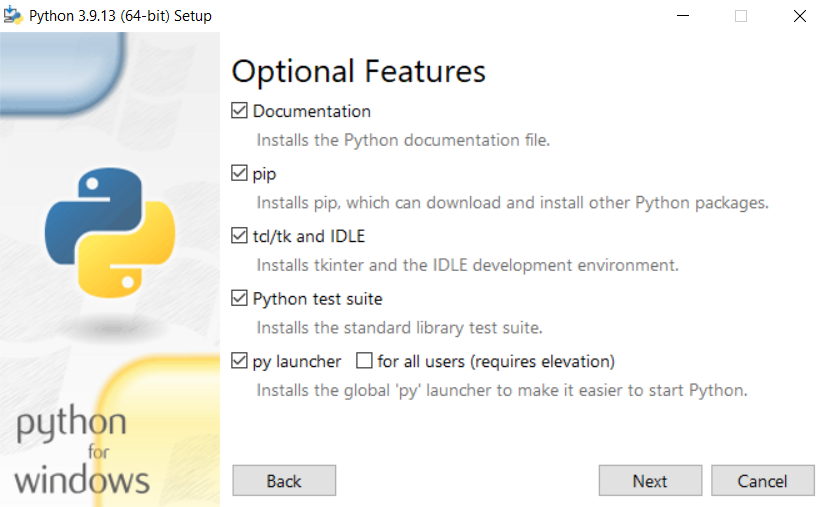
\includegraphics[width=.8\linewidth]{python_install3}%
			}		
			\medskip	
		\end{minipage}
		Choose Customize Installation, check option "Add Python to PATH" and decide if you want to install Python for all users, I prefer not to.
		\item \begin{minipage}[t]{\linewidth}
			\raggedright
			\adjustbox{valign=t}{%
				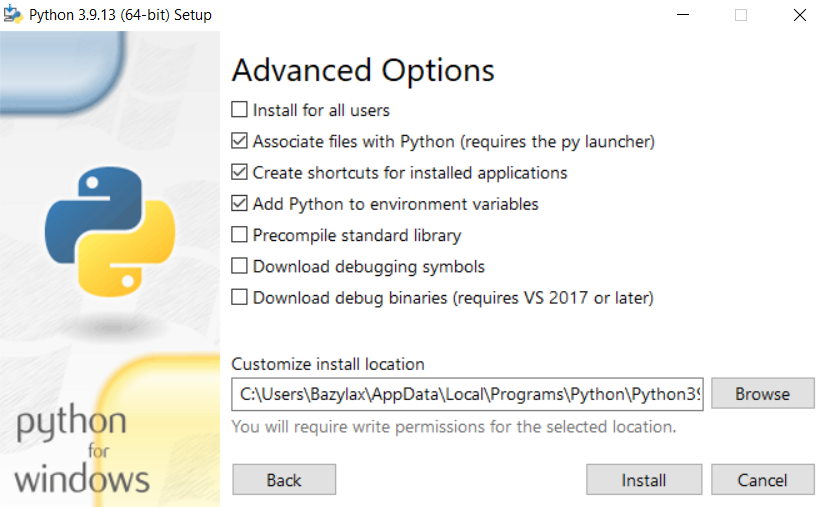
\includegraphics[width=.8\linewidth]{python_install4}%
			}		
			\medskip	
		\end{minipage}
		Leave everything checked and again decide whether to install it for all users.
		\item \begin{minipage}[t]{\linewidth}
			\raggedright
			\adjustbox{valign=t}{%
				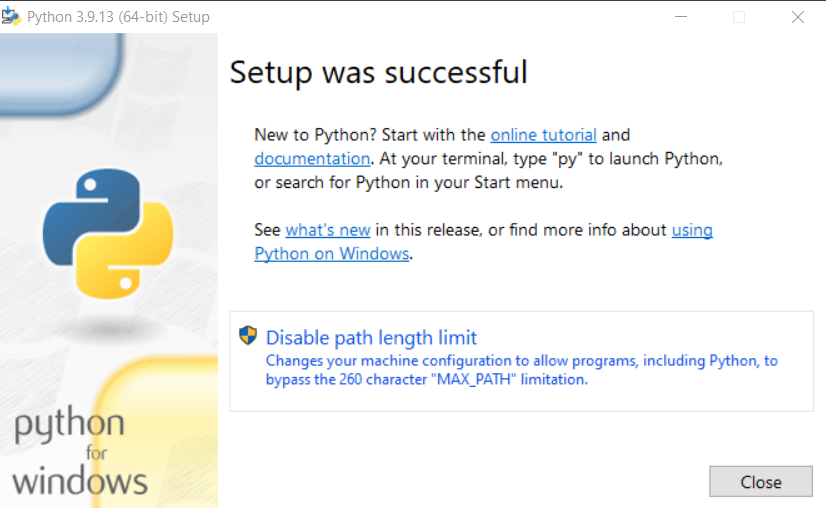
\includegraphics[width=.8\linewidth]{python_install5}%
			}		
			\medskip	
		\end{minipage}
		Choose options as in the picture above and if you wish change the install location and click install. In the ending screen you can choose to disable PATH length limit, but that requires admin permissions.
		\item To check if python was installed properly write "python" in cmd, this should display python version and enable python console. To quit write Ctrl+Z and press Enter. If it doesn't work or Microsoft Store with Python to download opens try following steps:
		\begin{itemize}
			\item Press Windows+R and type "sysdm.cpl", window will pop up, then press "Advanced" and there press "Environment variables".
			\item \begin{minipage}[t]{\linewidth}
				\raggedright
				\adjustbox{valign=t}{%
					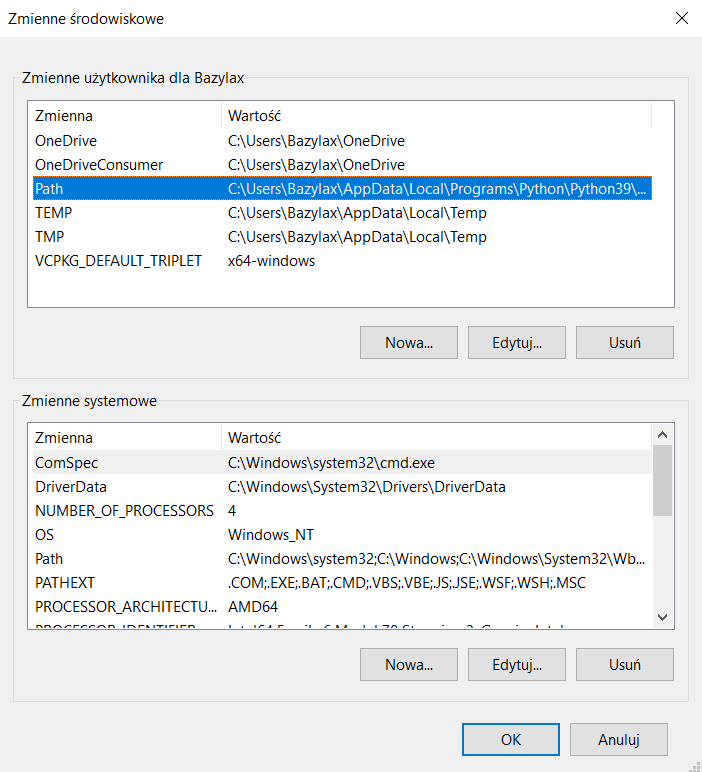
\includegraphics[width=.8\linewidth]{python_install6}%
				}		
				\medskip	
			\end{minipage}
			Window as above should pop up, click on the Path.
			\item \begin{minipage}[t]{\linewidth}
				\raggedright
				\adjustbox{valign=t}{%
					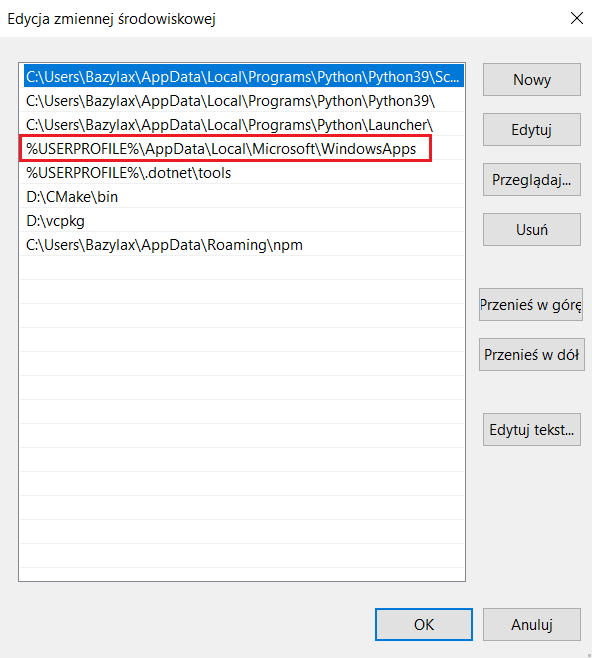
\includegraphics[width=.8\linewidth]{python_install7}%
				}		
				\medskip	
			\end{minipage}
			Make sure that all paths containing Python are above selected path to WindowsApps. If not, move them above WindowsApps path.
		\end{itemize}
	\end{itemize}
	\item Install IDE (Integrated Development Environment) of your choice, I will provide installation instruction for PyCharm:
	\begin{itemize}
		\item Go to \url{https://www.jetbrains.com/pycharm/download/?section=windows}
		\item \begin{minipage}[t]{\linewidth}
			\raggedright
			\adjustbox{valign=t}{%
				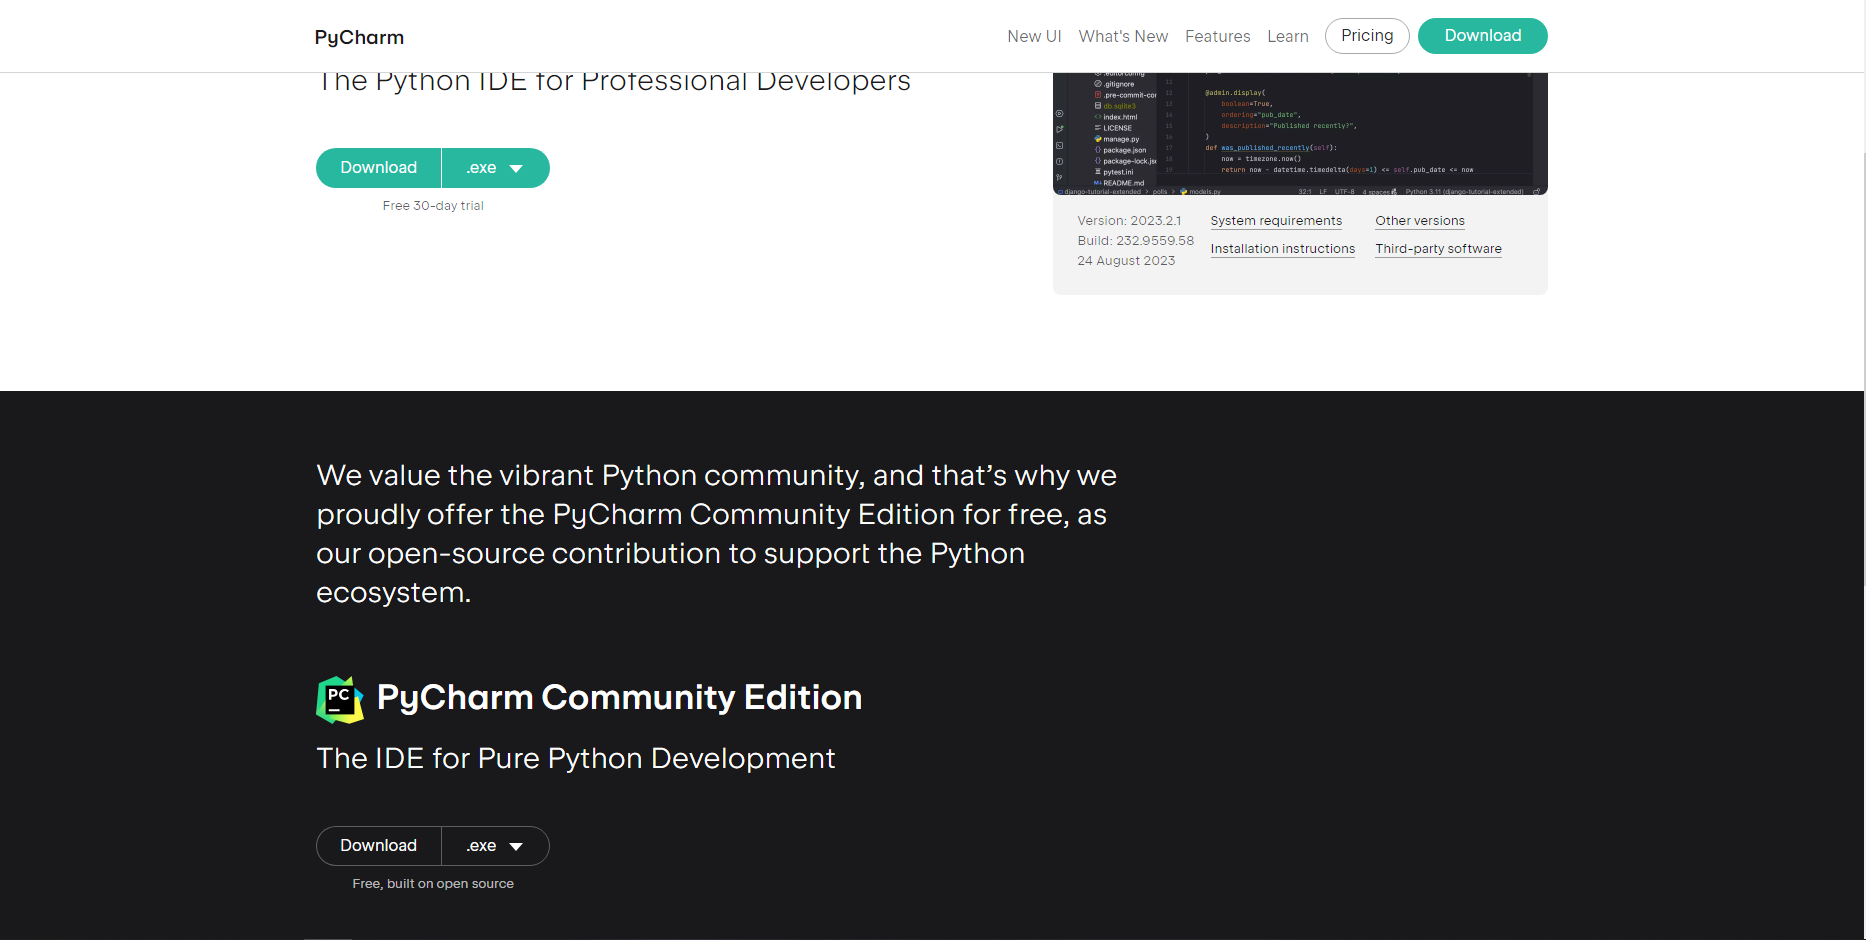
\includegraphics[width=.8\linewidth]{pycharm_install1}%
			}		
			\medskip	
		\end{minipage}
		Scroll down to download free Community Edition and click download button.
		\item \begin{minipage}[t]{\linewidth}
			\raggedright
			\adjustbox{valign=t}{%
				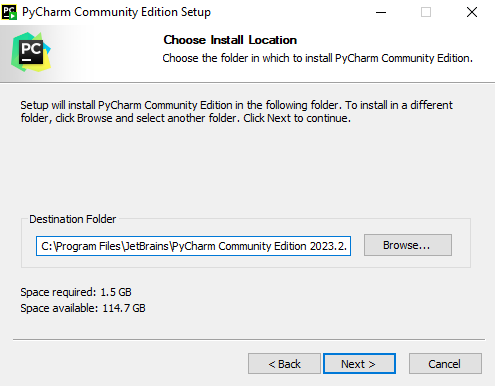
\includegraphics[width=.8\linewidth]{pycharm_install2}%
			}		
			\medskip	
		\end{minipage}
		Run the installer and choose install location.
		\item \begin{minipage}[t]{\linewidth}
			\raggedright
			\adjustbox{valign=t}{%
				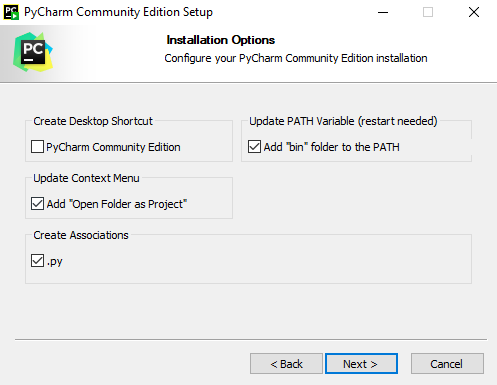
\includegraphics[width=.8\linewidth]{pycharm_install3}%
			}		
			\medskip	
		\end{minipage}
		Choose options as above as they grant conveniency of usage, create desktop shortcut as you'd like.
		\item Then just click Install.
	\end{itemize}
	\item If you had followed telemetry-extraction manual, you should have a folder containing \verb|Frames_extractor| and GoPro-Telemetry-Extractor. If you don't have them, check the manual of telemetry extractor. Now copy the contents of GoPro-Telemetry-Extractor and move them to \verb|Frames_extractor| folder. 
	\linebreak	
	\item Create new PyCharm project in \verb|Frames_extractor| folder and use existing files:
		\begin{itemize}
			\item \begin{minipage}[t]{\linewidth}
				\raggedright
				\adjustbox{valign=t}{%
					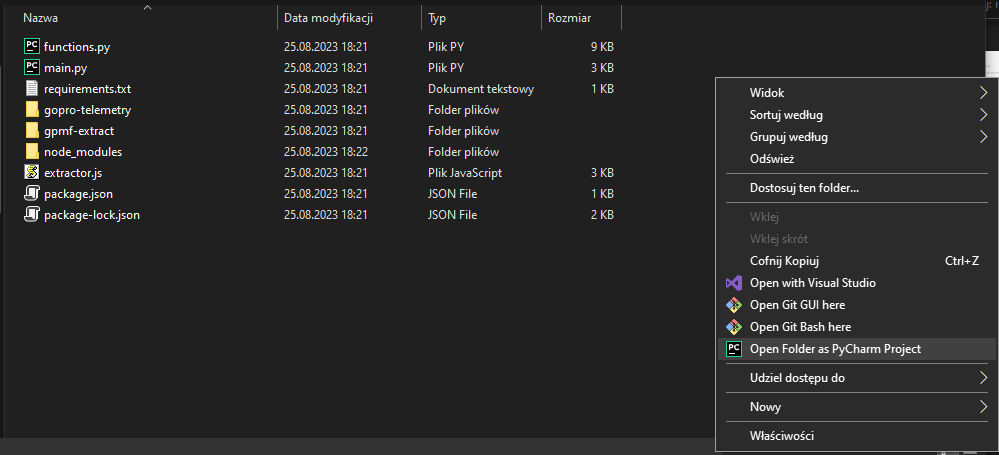
\includegraphics[width=.8\linewidth]{run1}%
				}		
				\medskip	
			\end{minipage}
			When in \verb|Frames_extractor| folder right-click and choose Open as PyCharm Project.
			\item \begin{minipage}[t]{\linewidth}
				\raggedright
				\adjustbox{valign=t}{%
					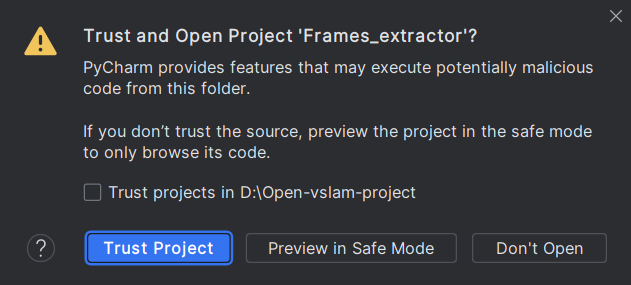
\includegraphics[width=.8\linewidth]{run2}%
				}		
				\medskip	
			\end{minipage}
			A windows asking us how we would like to open the project should pop up, just click Trust Project.
			\item \begin{minipage}[t]{\linewidth}
				\raggedright
				\adjustbox{valign=t}{%
					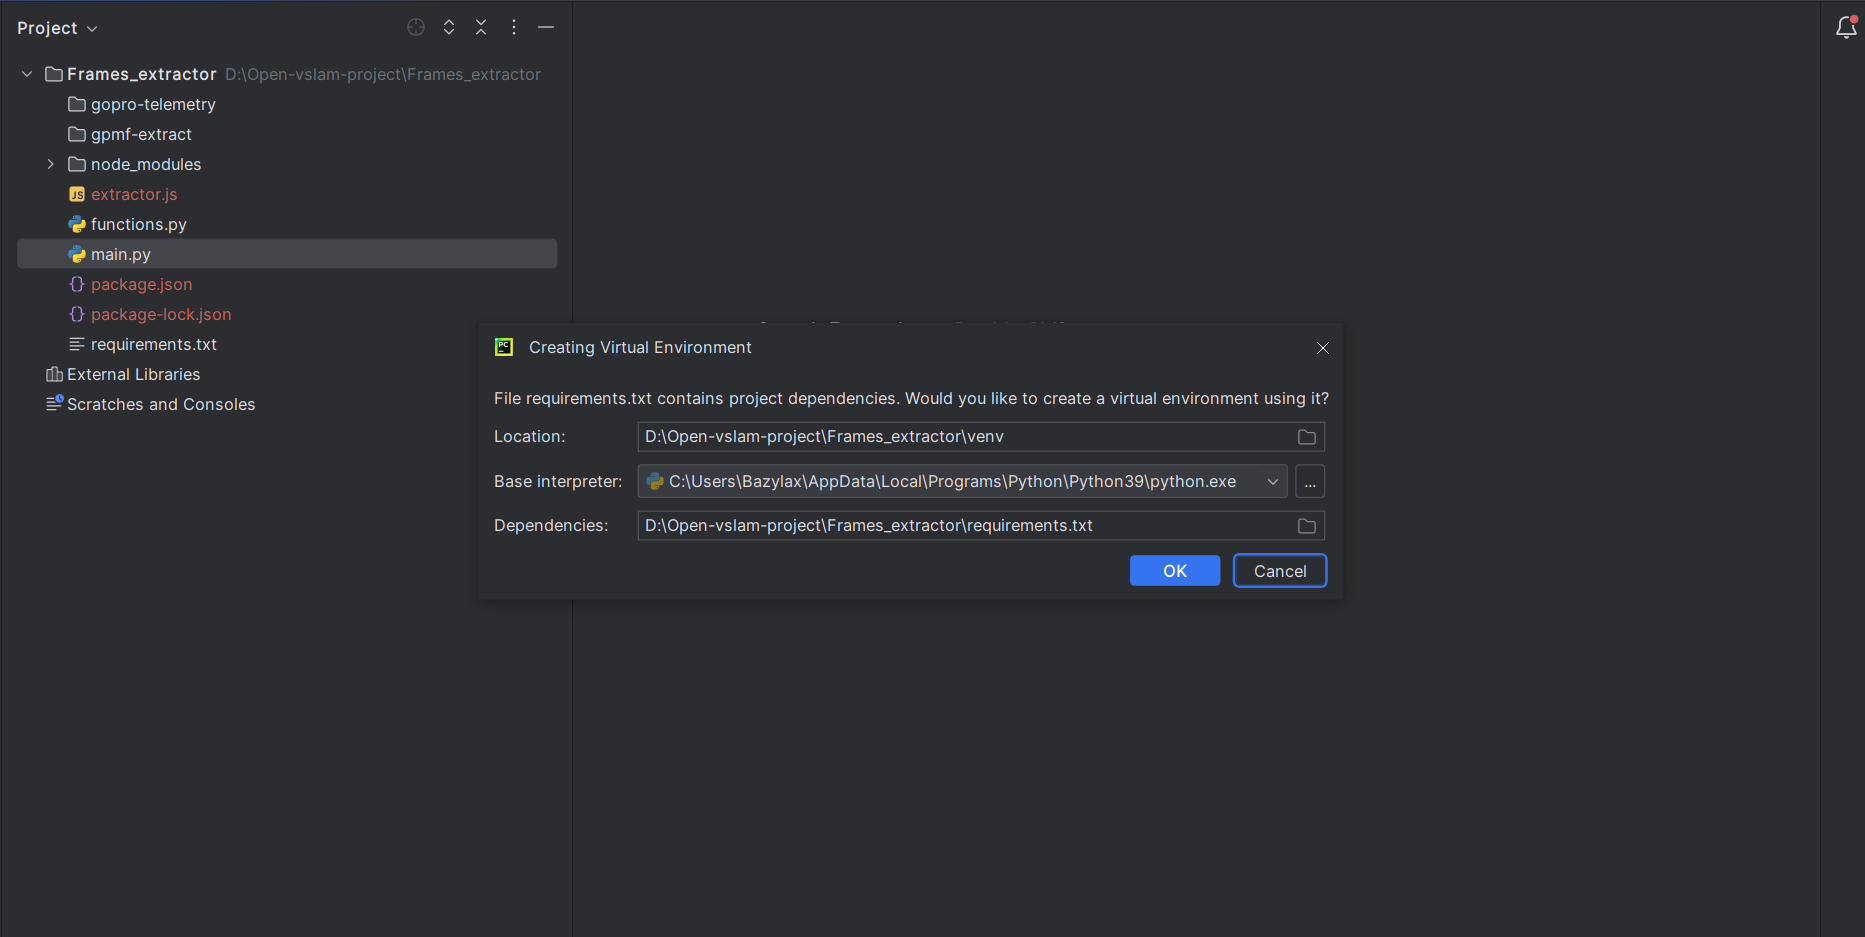
\includegraphics[width=.8\linewidth]{run3}%
				}		
				\medskip	
			\end{minipage}
			Now we create virtual environment in the same folder, interpreter should be python that was installed earlier and dependencies the requirements.txt file. Click ok if everything is set.
			\linebreak
			\item \begin{minipage}[t]{\linewidth}
				\raggedright
				\adjustbox{valign=t}{%
					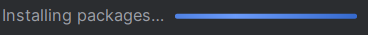
\includegraphics[width=.8\linewidth]{run4}%
				}		
				\medskip	
			\end{minipage}
			On the bottom of the screen you should see loading bar informing about building virtual environment and installing packages. When it finishes open main.py and run it.
		\end{itemize}		
	 \item \begin{minipage}[t]{\linewidth}
		\raggedright
		\adjustbox{valign=t}{%
			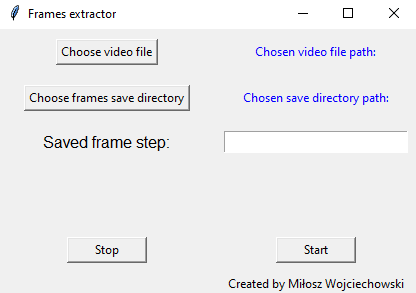
\includegraphics[width=.8\linewidth]{window1}%
		}		
		\medskip	
	\end{minipage}
	After running main.py application window should open.
	There can be seen a few buttons and an input area:
	\begin{itemize}
		\item \textbf{Choose video file} - open file explorer and select video file. As opposed to telemetry extractor it is recommended to avoid .LRV file since extracted frames should be the highest possible quality.
		\item \textbf{Choose Frames save director}y - open file explorer and choose directory which extracted frames will be saved to. Make sure chosen folder is empty or create a new empty one.
		\item \textbf{Saved frame step} - defines how many frames will pass between those extracted e.g. when set to 30 program will extract one frame after every 30 frames. So for video recorded in 30 FPS program will extract a frame every one second.
		\item \textbf{Start} - run the program, before that make sure you filled all the needed data (video file, save directory and frame step). The output of the program will be: telemetry-data.csv, folder with extracted frames and html map visualization.
		\item \textbf{Stop} - button to stop frames extracting process while it is running.
	\end{itemize}
	\item \begin{minipage}[t]{\linewidth}
		\raggedright
		\adjustbox{valign=t}{%
			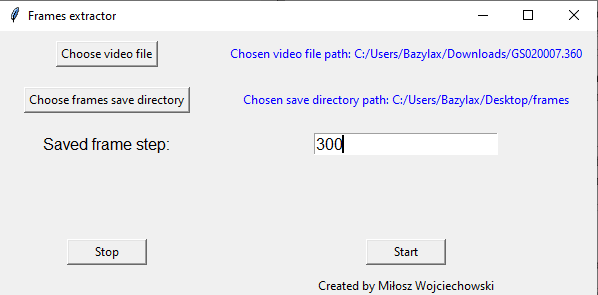
\includegraphics[width=.8\linewidth]{window2}%
		}		
		\medskip	
	\end{minipage}
	After filling all the needed data press "Run" button. Frames will be extracted to provided location, csv file with telemetry data will appear in the folder with main.py file and the map will open. Don't close the application window until being finished with using visualization.
\end{enumerate}
\end{document}